%!TEX root = ../../main.tex

\chapter{Grundlagen}
\label{chapter:3}

\section{Humanzentriertes Design}

Beim Entwickeln neuer Software setzen erfahrene Softwareentwickler häufig auf einen gut durchdachten Plan und Struktur. Dabei wird auf bestimmte Entwicklerprozesse gesetzt. Einer der bekanntesten Prozesse in der Softwareentwicklung ist hierbei der “Software Development Lifecycle” (kurz: SDLC). Der SDLC wird genutzt, um möglichst effiziente, kostengünstige Software mit hoher Qualität zu designen, entwickeln und produzieren1. Es gibt eine Menge verschiedene Modelle des SDLC, jedoch haben alle Modelle im Grunde dieselbe Struktur: Planen – Designen – Implementieren – Testen. Besonders auf den Baustein “Design” soll in diesem Kapitel tiefer eingegangen werden.

Eine der weitverbreitetsten Designmodelle ist das “Human Centered Design” (kurz: HCD, dt.: menschenzentriertes Design).  Dabei handelt es sich um eine Designtechnik, bei der der Mensch im Vordergrund des Entwicklungsprozesses steht.2 Laut der Webseite der Harvard Business School liegen die Ziele des HCD darin, die Ziele, Wünsche und Vorlieben des Produktnutzers stetig im Auge zu behalten.3 Dort beschreibt ein Dekan der Harvard Business School vier grundlegende Phasen im HCD. Diese sind laut Dekan Srikant Datar folgende Phasen: Clarify – Ideate – Develop – Implement.4 Wiederum definiert Sim van der Ryn in seinem Paper “Human Centered Design” aus dem Jahr 2013 das Vorgehen des HCD ein wenig anders, jedoch ähnlich. Dieser schreibt, dass man sich zuerst mit dem potenziellen Nutzer beschäftigen sollte.5 Anschließend wird das Problem definiert, eine Idee erarbeitet, ein Prototyp erstellt und abschließend getestet.6

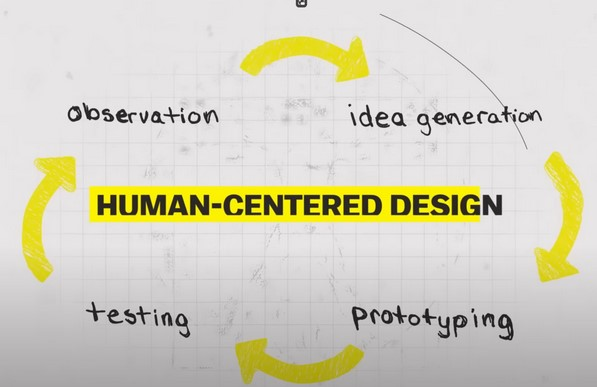
\includegraphics[width=1\textwidth]{images/03/HCD.jpg}


Zu den Vorteilen des HCD gehören unter anderem eine hohe Nutzerzufriedenheit, da die Meinung von Personen unmittelbaren Einfluss auf das Design des Produkts nehmen und so sicherstellen, dass alle Bedürfnisse und Erwartungen an das Produkt garantiert werden.7 Zudem kann dadurch auf die Wechselwirkung zwischen Menschen und Objekten besser verstanden werden, da man durch die Designfrage wichtige Erkenntnisse über das Verhalten bzw. Bedürfnisse der Menschen oder zumindest einer Personengruppe bekommt.8

Jedoch gibt es auch einige Nachteile bzw. Probleme des HCD. Ein Aspekt wäre die rapide Produktlebenszyklus. Durch die ständig wechselnden Bedürfnisse und Anforderungen an ein Produkt, stehen Designer und Designteams ständig unter großen Herausforderungen, um die Ansprüche treffen zu können.9 Häufig könnten aber auch eben diese menschlichen Anforderungen an ein Produkt zum Problem werden, da diese Anforderungen nicht umsetzbar und realisierbar sind.10


% TODO: die vlt einarbeiten oder sind die sachen schon drin ?
% > hier kann man dann einfach Human Centered Design erklären
% > Man könnte vlt das Prinzip auch mit dieser “Norman Door” erklären und dem leser ein wenig verinnerlichen so und das selbst so ein einfaches Prinzip von einer Türe schon so komplex sein kann. Das dass anpassen einer Webseite extrem schwer ist für den Nutzer
% Erklären was das ist was für variaten es gibt und wie das generelle vorgehen davon vlt sein kann
% It's not you. Bad doors are everywhere. - YouTube
% > Discoverability
% > Feedback

\subsection{Definition und Prinzipien des Humanzentrierten Designs}

\subsection{Anwendung von Humanzentriertem Design im Webkontext}

\section{Webtechnologien}

\subsection{Verwendung von React und anderen Webtechnologien in der App-Entwicklung}

\subsection{Technische Grundlagen der CO2-Runter-App}
